\chapter{Conceptos clave}

\section{Paramics}
\section{OMNeT++}
\section{TraCI}
TraCI (\textbf{Tra}ffic \textbf{C}ontrol \textbf{I}nterface) es una arquitectura para la interacción con simuladores de redes de transporte, cuyo principal propósito es facilitar el diseño y la implementación de simulaciones de Sistemas de Transporte Inteligente \cite{traci}. Proporciona una interfaz unificada que permite no sólo la obtención de datos desde la simulación de transporte, sino que también permite el control directo sobre la ejecución de ésta y provee métodos para la modificación del comportamiento de sus componentes. Así, TraCI permite a un agente externo (como, por ejemplo, un simulador de redes) comunicarse de manera bidireccional con la simulación de la red de transporte, posibilitando un desarrollo dinámico de dicha simulación en reacción a estímulos externos.

Hoy en día, dicha arquitectura se encuentra integrada con SUMO, y se utiliza en conjunto con simuladores de redes de comunicación inalámbrica como OMNeT++ y NS2 para la simulación y estudio de Sistemas de Transporte Inteligente.

\subsection{Diseño}
\subsubsection{Mensajes}

TraCI se basa en una arquitectura cliente-servidor, en la cual el simulador de redes de transporte asume el rol de un servidor pasivo que espera comandos desde un cliente activo. Define además un protocolo de comunicaciones de capa de aplicación para la transmisión de comandos e información entre servidor y cliente mediante un \emph{socket} TCP.

La figura \ref{fig:traci_msg:command} ilustra la estructura básica de un mensaje TraCI enviado desde un cliente al servidor. Consiste en una cadena de comandos TraCI consecutivos que deben ser ejecutados por este último; cada comando tiene un largo y un identificador, y puede incluir información adicional -- por ejemplo, en el caso de que se trate de un comando que asigne algún valor a una variable de la simulación. En caso de que el valor del largo exceda 255, este se fija en \texttt{0x00} y se agrega un campo de 32 bits para almacenar dicho valor.

Por otro lado, la figura \ref{fig:traci_msg:response} ilustra un ejemplo de respuesta del servidor, el cual debe responder a cada uno de éstos mensajes con una notificación del estado de la solicitud (``OK'', ``ERROR'' o ``NO IMPLEMENTADO'') y, en caso de que corresponda, con información adicional de acuerdo a parámetros específicos definidos para cada comando. Finalmente, la figura \ref{fig:tracigetversion} ilustra el flujo de mensajes para la solicitud de una variable de la simulación.

\begin{figure}[t]
    %\centering
    \begin{subfigure}{.3\textwidth}
        \centering
        \begin{bytefield}{16}
            \bitheader{0,7,8,15} \\
            \begin{rightwordgroup}{Cabecera}
                \wordbox{2}{Largo del mensaje, incluyendo la cabecera}
            \end{rightwordgroup} \\
            \begin{rightwordgroup}{Comando 0}
                \bitbox{8}{Largo} & \bitbox{8}{ID Comando} \\
                \wordbox{1}{Parámetros del Comando}
            \end{rightwordgroup} \\
            \begin{rightwordgroup}{Comando 1\\(Ejemplo\\largo ext.)}
                \bitbox{8}{0x00} & \bitbox[lrt]{8}{}\\
                \wordbox[lr]{1}{Largo extendido (32 bits)}\\
                \bitbox[lrb]{8}{} & \bitbox{8}{ID Comando} \\
                \wordbox{1}{Parámetros del Comando}
            \end{rightwordgroup} \\
            \wordbox[]{1}{$\vdots$} \\[1ex]
            \begin{rightwordgroup}{Comando n}
                \bitbox{8}{Largo} & \bitbox{8}{ID Comando} \\
                \wordbox{1}{Parámetros del Comando}
            \end{rightwordgroup} \\
        \end{bytefield}
        \caption{Comandos}
        \label{fig:traci_msg:command}
    \end{subfigure}\hspace{0.2\textwidth}%
    \begin{subfigure}{.3\textwidth}
        \centering
        \begin{bytefield}{16}
            \bitheader{0,7,8,15} \\
            \begin{rightwordgroup}{Cabecera}
                \wordbox{2}{Largo del mensaje, incluyendo la cabecera}
            \end{rightwordgroup} \\
            \begin{rightwordgroup}{Estatus\\Comando 0}
                \bitbox{8}{Largo} & \bitbox{8}{ID Comando} \\
                \bitbox{8}{Estatus} & \bitbox[lrt]{8}{} \\
                \wordbox[lrb]{1}{Descripción}
            \end{rightwordgroup}\\
            \begin{rightwordgroup}{Respuesta\\Comando 0\\(Opcional)}
                \bitbox{8}{Largo} & \bitbox{8}{ID Respuesta} \\
                \wordbox{2}{Respuesta a comando}
            \end{rightwordgroup} \\
            %            \begin{rightwordgroup}{Comando 1}
            %                \bitbox{8}{0x00} & \bitbox[lrt]{8}{}\\
            %                \wordbox[lr]{1}{Largo extendido (32 bits)}\\
            %                \bitbox[lrb]{8}{} & \bitbox{8}{Identificador} \\
            %                \wordbox{1}{Parámetros del Comando}
            %            \end{rightwordgroup} \\
            \wordbox[]{1}{$\vdots$} \\[1ex]
            \begin{rightwordgroup}{Estatus\\Comando n}
                \bitbox{8}{Largo} & \bitbox{8}{ID Comando} \\
                \bitbox{8}{Estatus} & \bitbox[lrt]{8}{} \\
                \wordbox[lrb]{1}{Descripción}
            \end{rightwordgroup} \\
        \end{bytefield}
        \caption{Respuesta}
        \label{fig:traci_msg:response}
    \end{subfigure}
    \caption{Formatos de mensajes TraCI}  
    \label{fig:traci_msg}  
\end{figure}

\begin{figure}
    \centering
    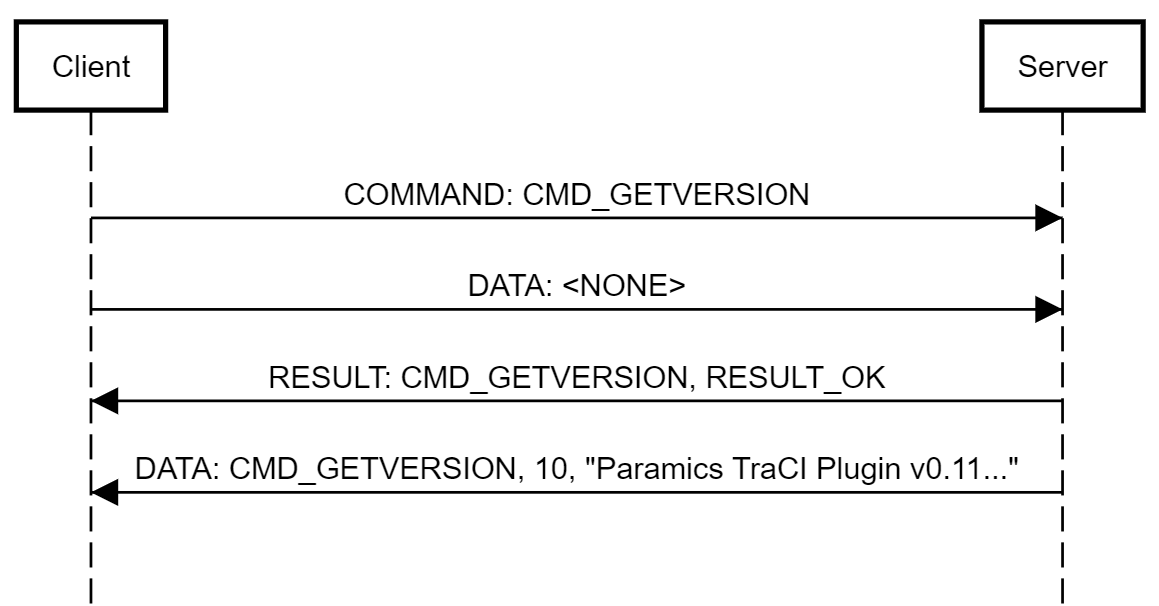
\includegraphics[width=1.0\linewidth]{imagenes/traci_getversion}
    \caption{Ejemplo de solicitud de variable TraCI.}
    \label{fig:tracigetversion}
\end{figure}


\subsubsection{Comandos}

El protocolo define cuatro categorías de comandos disponibles:

\begin{itemize}
    \item \textbf{Control de Simulación:} Esta categoría abarca en total tres comandos distintos, relacionados directamente con el control de la ejecución de la simulación:

    \begin{description}
        \item [\texttt{0x00 GET VERSION}] Por diseño, es el primer mensaje en ser enviado por el cliente al iniciar una sesión TraCI -- esto para asegurar versiones compatibles del protocolo con el servidor. Este último debe retornar un byte indicando la versión implementada de la API de TraCI y un \emph{string} opcional de descripción del software.
        
        \item [\texttt{0x02 SIMULATION STEP}] Corresponde al comando de control de simulación fundamental del protocolo, a través del cual el cliente controla la ejecución de cada paso de la simulación en el servidor.
        
        Este comando tiene dos modos de operación; \emph{single step} y \emph{target time step}. En en el modo \emph{single step}, el servidor ejecuta exactamente un único instante de tiempo en la simulación, mientras que en el \emph{target time step} el cliente le indica un instante de tiempo ``objetivo'' $T$, y el servidor ejecuta cuantos pasos sean necesarios tal que la simulación alcance el menor instante de tiempo $t$ tal que $t \geq T$. En ambos modos, luego de avanzar la simulación, el servidor debe retornar las ``suscripciones'' que el cliente haya solicitado con anterioridad. Estas consisten en conjuntos de datos que el cliente puede requerir luego de cada ejecución de la simulación (por ejemplo, las posiciones de todos los vehículos de la simulación).
        
        \item [\texttt{0x7f CLOSE}] Este mensaje es enviado por el cliente cuando desee cerrar la conexión y finalizar la simulación. El servidor entonces anuncia la recepción del comando y procede a cerrar el socket.
    \end{description}
    
    \item \textbf{Obtención de Valores:} Esta categoría abarca una gran cantidad de comandos asociados a variables internas de la simulación vehicular o de sus componentes (vehículos, cruces, etc.). Cada comando representa a un conjunto de variables específicas; por ejemplo, \texttt{0xa2 GET TRAFFIC LIGHTS VARIABLE} agrupa y obtiene los valores asociados a las variables propias de los semáforos en la red simulada, mientras que \texttt{0xa4 GET VEHICLE VARIABLE} está relacionado exclusivamente con los valores de los vehículos presentes en la red.
    
    \item \textbf{Modificación de Estados:} Finalmente, aquí se agrupan aquellos comandos que modifican valores y parámetros de la simulación y al igual que en la categoría anterior, cada comando de esta categoría está asociado a un conjunto de variables. Estos comandos tienden a ser más complejos que aquellos de categorías anteriores, ya que por razones obvias incluyen más información que debe ser interpretada por el servidor.    
\end{itemize}

